\pdfoutput=1

\documentclass{4thYearProject}

\makeatletter\@openrightfalse\makeatother
\usepackage{graphicx}
\usepackage{tabularx}
\usepackage{diagbox}
\usepackage{hyperref}
\usepackage{float}
\usepackage{longtable}
\usepackage{listings}
\usepackage{color}
\usepackage{pdfpages}

\definecolor{dkgreen}{rgb}{0,0.6,0}
\definecolor{gray}{rgb}{0.5,0.5,0.5}
\definecolor{mauve}{rgb}{0.58,0,0.82}

\newcolumntype{Y}{>{\raggedleft\arraybackslash}X}

\lstset{frame=tb,
  language=SQL,
  aboveskip=3mm,
  belowskip=3mm,
  showstringspaces=false,
  columns=flexible,
  basicstyle={\small\ttfamily},
  numbers=none,
  numberstyle=\tiny\color{gray},
  keywordstyle=\color{blue},
  commentstyle=\color{dkgreen},
  stringstyle=\color{mauve},
  breaklines=true,
  breakatwhitespace=true,
  tabsize=3,
  belowskip=1em
}

\graphicspath{ {resources/images/} }

\begin{document}
\title{Microissues IntelliJ Plugin !NAME TO BE CONSIDERED!}
\author{Alex Leet}
\date{2016/2017}
\maketitle

\begin{abstract}
Abstract here
\end{abstract}

\educationalconsent
%
%	NOTE: if you include the educationalconsent (above) and your project is graded an A then
%      it may be entered in the CS Hall of Fame
%
\tableofcontents
%==============================================================================

\chapter{Introduction}
\pagenumbering{arabic}

\section{Project Context}

Testing citation \cite{microissues}


\section{Motivation}


\section{Objectives}


\section{Achievements}


\section{Dissertation Structure}

Go over the structure of the dissertation.

\begin{table}[H]
\caption{Dissertation Structure}
\centering
\def\arraystretch{1.5}
\begin{tabular}{p{3cm}p{12cm}}
\hline
Chapter & Content \\
\hline
2. Background & A short description of the previous work related to the project. \\
3. Requirements & Discusses the gathering of the requirements, followed by a list of all requirements. \\
4. Design and Implementation & Describes the architecture of the plugin. Details the design decisions taken. Also contains a list of final design features.\\
5. Evaluation & Describes the test process and the user evaluation carried out, their results and a discussion of the results. \\
6. Conclusion: & Discusses the outcome of the project, future work possibilities and learning outcomes.  \\
\hline
\end{tabular}
\label{table:reportStructure}
\end{table}


\chapter{Background}

Text on what this chapter talks about

\section{Issue Tracking}

A short section on issue-tracking systems and what they are.

\section{Related Work}

Various plugins have been developed to ease the integration of development environments with issue management. However, as the below mentioned examples will demonstrate, most are intended to connect to the various issue management systems. 

\subsection{Inbuilt IntelliJ Task Management Plugin}

IntelliJ IDEA is bundled with its own task management plugin and is activated by default. It allows for integration to various issue tracking systems, which allows the user to open, create and delete tasks or issues. Therefore a server that the tasks and issues are hosted on is necessary to use the inbuilt feature, which means there is no capability to create tickets locally. Additionally, tickets cannot be linked to source code in any way.

\begin{figure}[H]
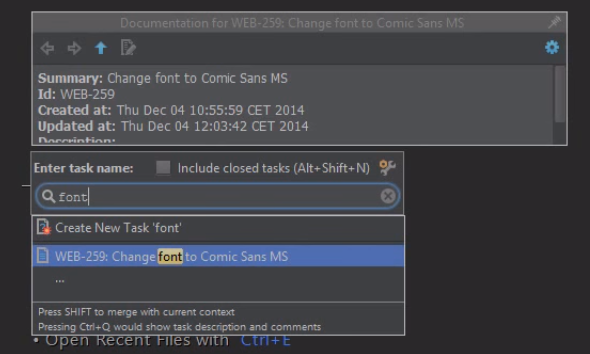
\includegraphics[scale=0.5]{IntelliJ_Tasks}
\centering
\caption{Example of viewing a YouTrack task in IntelliJ}\label{intellijtask}
\label{fig:intellijtask}
\end{figure}

\subsection{Tasks Navigation Plugin}

An attempt to connect source code to issue management systems in order to reduce context switch was attempted by Vladislav Rassokhin, who developed the plugin "Tasks Navigation" that allows the user to link to tasks (issues) in the Web from comments and reference injections in IntelliJ \cite{tasksnavigation}. With the plugin it is easy to quickly get information about the issue and to see which 

\begin{figure}[H]
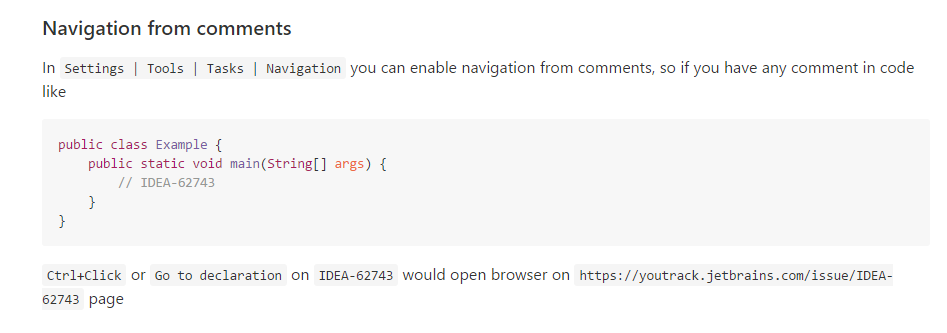
\includegraphics[scale=0.6]{Tasks_Navigation_Plugin}
\centering
\caption{Example of how the Tasks Navigation plugin works}\label{tasksnavigation}
\label{fig:tasksnavigation}
\end{figure}

\subsection{Tasks Plugin}

Another IntelliJ plugin that was developed by Sergiy Dubovik and continued by Warner Jan Veldhuis is Tasks, which allows the user to locally manage tasks and issues. The plugin includes the ability to assign priority to tasks and keep track for how long they have been worked on. However, there is no possibility to connect the tasks to source code. 

\begin{figure}[H]
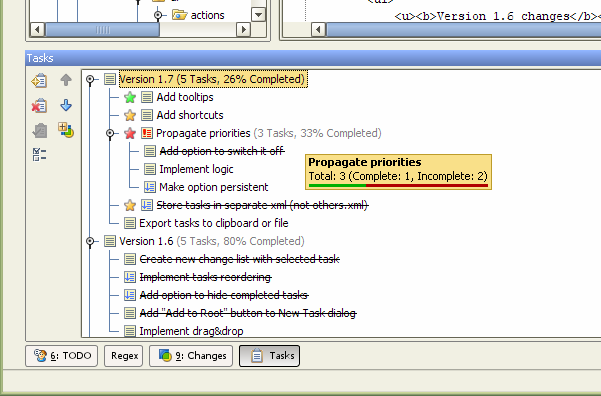
\includegraphics[scale=0.6]{Tasks}
\centering
\caption{Example of task management in the Tasks plugin}\label{tasks}
\label{fig:tasks}
\end{figure}

\subsection{Mylyn}

Mylyn is the task and application lifecycle management (ALM) framework for Eclipse. 

\subsection{Eclipse TODO Editor Plugin}

The Eclipse todo editor plugin that allows to edit todo files in Eclipse. 

\begin{figure}[H]
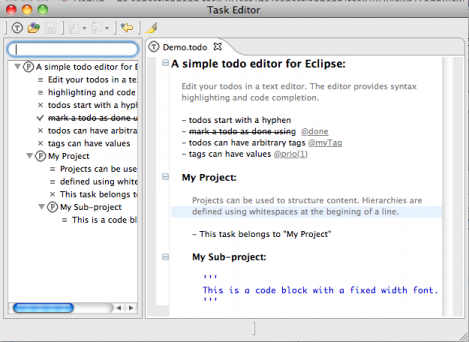
\includegraphics[scale=0.6]{eclipse_TODO_editor}
\centering
\caption{Example of the editor window, including the visual display of todo's on the left}\label{eclipsetodo}
\label{fig:eclipsetodo}
\end{figure}

\subsection{Summary of Related Work}

\begin{center}

\noindent
\begin{tabular}{|l||*{5}{c|}}\hline
\backslashbox[50mm]{Plugin}{Feature}
&\makebox{Integration with source code}&\makebox{Local issue management}&\makebox{Display of all issues}
\\\hline
IntelliJ Inbuilt Plugin & Yes &&\\\hline
Tasks Navigation & No &&\\\hline
Tasks & Yes &&\\\hline
Mylyn & No && \\\hline
Eclipse TODO Editor & Yes && \\\hline
\end{tabular}

\end{center}

\section{Research on Issue Tracking and Usage of Issue-tracking Systems}

Attemps have been made to research recording of issues and bugs and the common shortcomings of how bugs and issues are documented. A study by Jorge Aranda and Gina Venolia has found that one of the most crucial bits of information missing in issue management is links to source code and the change-sets that resolved these bugs \cite{lifeofbugs}. Additionally, they had found that in some cases, the key events in the story of a bug had left no electronic trace and therefore there was no way to discover the important information pertaining the fixing of a bug.

\section{Evaluation of Related Work and Related Research}

\chapter{Requirements}

\section{Requirements Elicitation and Gathering}


\section{Functional Requirements}

\newpage
\section{Non-Functional Requirements}

\chapter{Design and Implementation}

Discuss design choices, justifications and implementation.

\section{Iterations Overview}

Overview of the development iterations.

\section{User Interface}

\chapter{Evaluation}

Describe the aims of this chapter

\section{Unit Testing}
\section{Acceptance Testing}


\chapter{Conclusion}

\section{Project Outcome}

Outline the project outcome. 

\section{Learning Outcomes}


%%%%%%%%%%%%%%%%%%%%
%   BIBLIOGRAPHY   %
%%%%%%%%%%%%%%%%%%%%

\bibliographystyle{ieeetr}
\bibliography{resources/bibliography}

%%%%%%%%%%%%%%%%
%              %
%  APPENDICES  %
%              %
%%%%%%%%%%%%%%%%

\begin{appendices}
\end{appendices}

\end{document}
